\documentclass{article}
\usepackage[utf8]{inputenc}
\usepackage{amsmath}
\usepackage{amsthm}
\usepackage{graphicx}
\usepackage{geometry}
\usepackage{caption}
\usepackage{hyperref}
\usepackage{minted}
\usemintedstyle{manni}
\geometry{a4paper, portrait, margin=1in}

\theoremstyle{plain}
\newtheorem{thm}{Theorem}

\theoremstyle{definition}
\newtheorem{defn}{Definition} % definition numbers are dependent on theorem numbers
\newtheorem{exmp}{Example} % same for example numbers

\hypersetup{
    colorlinks=true,
    urlcolor=blue,
}

\title{Operating Systems (UE18CS302)\\
    \large Unit 2}
\author{Aronya Baksy}
\date{August 2020}

\begin{document}
    \maketitle
    
\section{Threads}
\begin{itemize}
    \item Threads are fundamental units of CPU execution, with each thread containing its own program counter, register set, stack and an identifier known as the \textbf{thread ID}.
    
    \item Processes contain single or multiple threads of execution. Multiple threads allow a process to perform multiple tasks at the same time (eg: most modern desktop applications like Web Browsers, Word Processors, spreadsheet programs etc. are multithreaded).
    
    \item Process creation is heavy and requires large overheads (mostly from context switching) while thread creation is lightweight with minimal overheads.
\end{itemize}

\subsection{Benefits of Multithreaded Programming}
\begin{itemize}
    \item \textbf{Responsiveness}: As threads are independent of each other, one can run even when another one is blocked (ie. waiting). This is useful in GUI applications where each thread can service one part of the UI and keep response times low. 
    
    \item \textbf{Resource Sharing}: Processes share resources using complicated IPC mechanisms, but threads can share resources easily as they use the memory address space of the process that created them. 
    
    \item \textbf{Economy}: Thread creation has minimal memory allocation and context switching overheads compared to process creation as threads share a common memory, while processes need their own memory and context.
    
    \item \textbf{Scalability}: A multi-threaded processes can run on multiple processing cores, while a single-threaded process can run only on one core (irrespective of how many cores are there in hardware). 
\end{itemize}
\begin{figure}
    \centering
    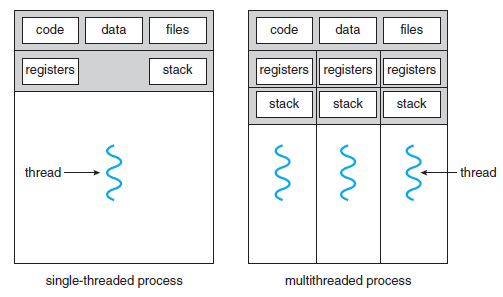
\includegraphics{os.png}
    \caption{Single and Multi-Threaded Architectures}
    \label{fig:my_label}
\end{figure}

\subsection{Multicore Programming (Concurrency vs Parallelism)}
\begin{itemize}
    \item Multithreaded programming provides a mechanism for more efficient use of these multiple computing cores and improved concurrency
    
    \item If an application has 4 threads, then on a single CPU system, the 4 threads will be interleaved but at a single instant, only one thread will be executed. 
    
    \item On a multicore system, a separate core can be assigned to run each thread, hence the threads can run in parallel. 
    
    \item \textbf{Concurrent} systems support the execution of more than one task, but only one task is executed at a single instant of time. 
    
    \item \textbf{Parallel} systems can execute multiple tasks at the same time, meaning that at a single isntance of time, there are $>1$ tasks running. 
    
    \item Concurrent systems can give the \textit{illusion} of being parallel with rapid and frequent switching between threads, but this is not true parallelism.
    
    \item Nowadays, all hardware manufacturers support multiple hardware threads per core (modern Intel and AMD CPUs have 2 threads per core)
\end{itemize}

\subsubsection{Amdahl's Law}
\begin{itemize}
    \item \textbf{Amdahl's Law} states that the the speedup obtained from running a program with a fraction of serial code given by $S$ on $N$ computational units (cores) is given by
    \begin{equation}
        speedup = \frac{1}{S + \frac{1-S}{N}}
    \end{equation}
    
    \item Amdahl's law proposes that the serial portion of the program has a disproportionate effect on any performance gain derived from adding more cores. (as $n \rightarrow \infty$, $speedup \rightarrow \frac{1}{S}$)
    
    \item Some argue that Amdahl’s Law does not take into account the hardware performance enhancements used in the design of contemporary multicore systems.
\end{itemize}

\subsection{Programming Challenges}
\begin{itemize}
    \item \textbf{Identifying tasks} that are simple and independent within the program logic.
    
    \item \textbf{Balanced} workloads on all tasks. If some tasks are less valuabe to the final output, then it may not be worth the effort to run them on separate cores.
    
    \item \textbf{Data splitting} to run on multiple cores
    
    \item \textbf{Data dependencies} between threads. Threads must be synchronized to avoid problems with multiple threads writing to/reading from the same memory location.
    
    \item \textbf{Testing and debugging} is more complicated due to many different execution paths possible. 
\end{itemize}

\subsection{Types of Parallelism}
\begin{itemize}
    \item \textbf{Data-level} parallelism involves distributing the data into multiple cores and each thread (running on a core) does the same task on this subset of the data
    
    \item \textbf{Task-level} parallelism involves different threads doing different tasks, on either the same data or different data.
    
    \item Real world applications use a hybrid of both types of parallelism.
\end{itemize}

\section{Multithreading Models}
These are different models of establishing a relationship between \textbf{user} and \textbf{kernel} threads.
\subsection{Many-to-One Model}
\begin{itemize}
    \item Multiple user threads are mapped to a single kernel thread. 
    
    \item Thread management is done by the thread library in user space, hence it is efficient.
    
    \item However if one thread executes a blocking system call, then all the the threads must stop execution. 
    
    \item Also, multiple cores cannot be taken advantage of as only one kernel thread is present to access the kernel at a time, hence multiple user threads cannot run at the same time
    
    \item eg: Green threads on Solaris and early Java versions
\end{itemize}

\subsection{One-to-One Model}
\begin{itemize}
    \item One user thread is mapped to one kernel thread
    
    \item Greater concurrency as another thread can be made to run when one thread makes a blocking system call. Multiple threads can also run in parallel on multiprocessors.
    
    \item Since creating a user thread also means creating a corresponding kernel thread, the overheads are high, and the OS can restrict the number of user threads being created.
    
    \item eg: Linux, Windows family OSes
\end{itemize}

\subsection{Many-to-Many Model}
\begin{itemize}
    \item Multiple user threads are multiplexed to a smaller or equal number of kernel threads.
    
    \item The developer can create as many user threads as needed, and the corresponding kernel threads can run in parallel on multicore systems.
    
    \item If one thread does a blocking system call, another kernel thread can be scheduled to run. 
    
    \item In a\textbf{ two-level system}, many user threads are still multiplexed to a certain number of kernel threads, but user threads can also be \textbf{bound} to a kernel thread. (eg: Solaris $<$9)
\end{itemize}

\section{Thread Scheduling}
\begin{itemize}
    \item On systems that support user-level and kernel-level threads, the kernel-level threads and not processes are scheduled by the operating system. 
    
    \item In order to be scheduled, user threads need to be mapped to a kernel thread, although this mapping may not be direct but might be via a \textbf{lightweight process} (LWP). 
\end{itemize}
\subsection{Contention Scope}
\begin{itemize}
    \item On many-to-one and many-to-many implementations, the thread library schedules user threads onto available LWPs. This scheduling is called \textbf{Process Contention Scope} or PCS scheduling. 
    
    \item PCS is called so because competition for CPU now happens between user threads scheduled on one process.
    
    \item To decide which kernel thread should be scheduled onto the CPU, \textbf{System Contention Scope} or SCS scheduling is used. SCS scheduling is used among all the threads in the system. 
    
    \item PCS is done according to priority—the scheduler selects the runnable thread with the highest priority to run. 
    
    \item User-level thread priorities are set by the programmer and are not adjusted by the thread library, although some thread libraries may allow the programmer to change the priority of a thread. 
    
    \item PCS will typically preempt the thread currently running in favor of a higher-priority thread; however, there is no guarantee of time slicing among threads of equal priority.
\end{itemize}

\section{Thread Libraries}
\begin{itemize}
    \item Thread Libraries are APIs for developers to create and manage threads
    
    \item They may be implemented entirely at the user level (ie. the data structures and the code are all in user space) and no system calls are made.
    
    \item They may also be implemented with kernel support, ie. code and data structures are in kernel space, and function calls of this API involve system calls.
    
    \item The three main thread libraries in use today are \texttt{pthreads}, Windows Threads and the Java threading library (for applications running on the JVM). 
\end{itemize}
\subsection{\texttt{pthread} code example}
The following is a code example that launches a separate thread to compute the sum of the first n natural numbers. 
\begin{listing}[ht]
\centering
    \begin{minted}{c}
        #include<stdio.h>
        #include<pthread.h>
        
        void* runner(void* arg);
        int sum = 0;
        
        int main(int argc, char* argv[])
        {
            pthread_attr_t attr;
            pthread_t tid;
            
            int num = atoi(argv[1]);
            
            pthread_attr_init(&attr);
            pthread_create(&tid, &attr, runner, (void*)&num);
            pthread_join(&tid);
            
            printf("Sum = %d\n", sum);
        }
        
        void* runner(void* arg)
        {
            int n = *((int*)arg);
            for(int i=1; i<n; ++i)
                sum += i;
            pthread_exit(NULL);
        }
    \end{minted}
    \title{\texttt{pthread} code example}
\end{listing}

\begin{itemize}
    \item The \texttt{pthread\_attr\_t()} function is used to initialize the \texttt{pthread\_attr\_t} structure that holds the thread attributes.
    
    \item The \texttt{pthread\_create()} function takes in the \texttt{pthread\_t} structure, the attributes, the pointer to the function to be run on that thread (which must have signature of \texttt{void* function(void* arg)}) and the argument to be passed to the thread function.
    
    \item Inside the thread function, the \texttt{void*} is converted to \texttt{int} and the computation is done. At the end of the computation, the \texttt{pthread\_exit(NULL)} function call signifies the end of that thread and return of control back to the main process.
    
    \item The \texttt{pthread\_join(\&tid)} function is used to make the main process wait for the child thread called \texttt{tid} to finish executing. 
    
\end{itemize}

\section{Process Synchronization}
\begin{itemize}
    \item Process synchronization is required to avoid \textbf{race conditions}.
    
    \item A race condition is a situation where multiple threads or processes access the same data concurrently, and the final outcome is dependent on the order in which the processes/threads accessed the data. 
    
    \item Synchronization ensures that only one process can access the data at any instant in time
\end{itemize}

\subsection{The Critical-Section Problem}
\begin{itemize}
    \item In a system consisting of $n$ processes $ \{ P_0, P_1, P_2, ..., P_{n-1} \}$, each process has a region of code called the \textbf{critical section} where it performs operations like updating a global variables, updating a table or opening a file. 
    
    \item The important feature of the critical section is that when one process is executing its critical section, no other process is allowed to execute its critical section. That is, no two processes may execute their critical sections at the same time.
    
    \item Each processes requests entry into its critical process in the \textbf{entry section}, executes the critical section, and exits using the \textbf{exit section}. All other code in the process falls under the \textbf{remainder section}. 
    
    \item The problem statement is to design a protocol that the $n$ processes can use to coordinate their execution. 
    
    \item The solution to the critical-section problem has the following characteristics:
    \begin{itemize}
        \item It must ensure \textbf{mutual exclusion}, ie. make sure that if process $P_i$ is executing its critical section, then no other process is executing its own critical section.
        
        \item It must ensure \textbf{progress}. If no process is executing its critical section, and there are some processes that wish to enter their critical sections, then only processes that are not executing their remainder sections are eligible to be selected to run their critical section next, and this selection cannot be postponed indefinitely.
        
        \item In short, progress implies that if a process is not using the critical section, then it should not stop any other process from accessing it.
        
        \item \textbf{Bounded waiting}. Between a process requesting access to the critical section, and the granting of the request, there is a finite number of times that all other processes can access their critical sections.
        
        \item In other words, the waiting time for a process between request for access and actual access must not be infinite. 
        
        \item Read \href{https://stackoverflow.com/questions/33143779/what-is-progress-and-bounded-waiting-in-critical-section/33409854#33409854}{this link} for clear explanation. 
    \end{itemize}
    
    \item No assumptions are made about the \textbf{relative speed} of the processes, but it is assumed that all processes are executing at non-zero speed. 
    
    \item In kernel mode, there are many scopes for race conditions (eg: two processes simultaneously opening a file may cause a race condition in the file table maintained by the OS). 
    
    \item With \textbf{preemptive kernels}, a process can be preempted when it is running in kernel mode. This sort of kernel can have race conditions, and is more prone to race condition in SMP (Symmetric MultiProcessing) systems, as more than one kernel process may run on different processors. 
    
    \item In a \textbf{non-preemptive kernel}, a process has continuous control of the CPU until it blocks, waits or completes execution. This kernel design is free from race conditions as only one process is active in the kernel at a given instant of time. 
\end{itemize}

\subsection{Peterson's Solution}
\begin{itemize}
    \item This is a software-based solution to the critical-section problem.
    
    \item Peterson's Solution works for two processes $P_1$ and $P_2$ (which are represented as $P_i$ and $P_j$ where $j = 1-i$), and it assumes that the \texttt{load} and \texttt{store} machine instructions are \textbf{atomic}, ie. cannot be interrupted.
    
    \item The two process share two data items, \texttt{bool flag[2]} and \texttt{int turn}.
    
    \item The \texttt{turn} variable indicates which process' turn it is to enter the critical section, if the \texttt{turn == i} then process process $P_i$ is allowed to execute in the critical section. The \texttt{flag[2]} array indicates whether the process is ready to enter the critical section, so \texttt{flag[i]} is set to true when process $P_i$ is ready to enter its critical section. 
    
    \item To enter the critical section, process $P_i$ sets the value of \texttt{flag[i]} to true, and then changes the value of \texttt{turn} to $i$.
    
    \item If both processes want to enter the critical section, then they both attempt to overwrite the \texttt{turn} variable, and only one edit survives (the other one takes place and then almost immediately gets overwritten), hence only that process gets permission to enter the critical section.
\end{itemize}
\begin{figure}[!ht]
 \begin{minipage}{0.5\textwidth}
  \centering
  \begin{minted}{c}
   do{
        flag[0]=true;
        turn = 1;
        while(flag[1]==true && turn ==1)
            ; //Busy Waiting
        //Critical Section
        
        flag[0] = false;
        
        //Remainder Section
   }while(true);
  \end{minted}
  \title{Code for Process $P_0$}
 \end{minipage}
 \begin{minipage}{0.5\textwidth}
  \centering
  \begin{minted}{c}
  do{
        flag[1]=true;
        turn = 0;
        while(flag[0]==true && turn ==0)
            ; //Busy Waiting
        //Critical Section
        
        flag[1] = false;
        
        //Remainder Section
   }while(true);
  \end{minted}
  \title{Code for Process $P_1$}
 \end{minipage}
\end{figure}
\subsubsection{Validity of Peterson's Solution}
\begin{itemize}
    \item The process $P_i$ will be inside its critical section when \texttt{flag[j]} is false (meaning that $P_j$ has left the critical section) or \texttt{turn == i} (meaning that $P_j$ is waiting for its turn to enter the critical section). 
    
    \item Hence, if both process are in their critical section, then this must imply that turn=0 and turn=1 are both true at the same time, which is not possible. Hence \textbf{mutual exclusion} is ensured.
    
    \item \textbf{Bounded waiting} is ensured as no process waits more than one turn to get control of its critical section.
    
    \item  A process cannot immediately re-enter the critical section if the other process has set its flag to say that it would like to enter its critical section. Hence Peterson's Algorithm also ensures \textbf{progress}.
    
    \item As Peterson's Algorithm ensures all 3 conditions, it can be considered as a valid solution to the Critical Section Problem.
\end{itemize}

\subsubsection{Drawbacks of Peterson's Solution}
\begin{itemize}
    \item The algorithm assumes that all load and store operations at the hardware level are \textit{atomic}, ie. they cannot be interrupted. On modern multiprocessor systems this assumption does not hold.
    
    \item Peterson's Solution also is hard to implement for more than two processes, and when it is extended for more than 2 processes it fails to guarantee bounded waiting.
\end{itemize}

\subsection{Hardware Synchronization: Locking}
\begin{itemize}
    \item In contrast to the software solution presented above, most modern systems expose APIs to application and kernel programmers which use the principle of \textbf{locking}.
    
    \item In non-preemptive kernels, the critical-section problem is solved by a primitive form of locking where no interrupt is allowed to occur while a shared variable is being modified (ie. some process is in its critical section). 
    
    \item This is not a feasible solution for multiprocessor systems as it reduces the performance and can cause timing issues with the CPU clock (while relies on interrupts to refresh itself).
    
    \item In most modern hardware platforms, the \texttt{test\_and\_set()} and \texttt{compare\_and\_swap()} instructions are provided as \textbf{atomic} (ie. non-interruptable) instructions. 
\end{itemize}

\subsubsection{Test and Set}
\begin{itemize}
    \item The test-and-set instruction is implemented as below
\end{itemize}
    \begin{listing}[ht]
    \centering
    \begin{minted}{c}
        bool test_and_set(bool* target){
            bool return_value = *target;
            *target = true;
            return return_value;
        }
    \end{minted}
    \title{\texttt{test\_and\_set()} implementation}
    \end{listing}
\begin{itemize}
    \item This instruction is an \textbf{atomic} instruction, meaning that if two test-and-set instructions are executed simulatenously on different CPUs, then they will be executed one after the other in some arbitrary order.
    
    \item Mutual exclusion can be implemented using the test-and-set instruction as shown below.
    The shared Boolean variable \texttt{lock} has an initial value of \texttt{false}.
\end{itemize}

\begin{figure}[h]
    \centering
        \begin{minted}{c}
            do{
                while(test_and_set(&lock))
                    ; //Do nothing
                //Critical Section
                lock = false;
                //Remainder Section
            }while(true);
        \end{minted}
        \title{Process structure using \texttt{test\_and\_set()}}
\end{figure}

\subsubsection{Compare and Swap}
\begin{itemize}
    \item The compare-and-swap instruction is implemented as below
\end{itemize}
\begin{figure}[h]
    \centering
    \begin{minted}{c}
        int compare_and_swap(int* value, int expected, int new_val){
            int temp = *value;
            if(temp==expected)
                *value = new_val;
            return temp;
        }
    \end{minted}
    \texttt{\texttt{compare\_and\_swap()} implementation}
\end{figure}

\begin{itemize}
    \item The compare-and-swap instruction compares the value present at the location of \texttt{value} and then changes the value to \texttt{new\_val} only if the value matches the expected value. 
    
    \item The process is implemented as below
\end{itemize}
\begin{figure}[!h]
    \centering
    \begin{minted}{c}
        do{
            while(compare_and_swap(&lock, 0, 1) != 0)
                ;  //Do nothing
            //Critical Section
            lock = 0;
            //Remainder Section
        }while(true);
    \end{minted}
    \title{Process structure using \texttt{compare\_and\_swap()}}
\end{figure}

\begin{itemize}
    \item The above algorithms satisfy mutual exclusion but do not satisfy bounded waiting. 
    
    \item For this a new solution is presented that satisfies all the three conditions, and maintains the variables \texttt{boolean lock;} and \texttt{boolean waiting[n];} where n is the number of processes. 
    
    \item This implementation is given below
\end{itemize}

\begin{figure}[!ht]
    \centering
    \begin{minted}{c}
        do{
        waiting[i] = true;
        key = true;
        while(waiting[i] == true && key == true)
            key = test_and_set(&lock);
        waiting[i] = false;
        
        /* Critical Section */
        
        j = (i+1)%n;
        while(j != i && !waiting[j])
            j = (j+1)%n;
        if(j==i)
            lock = false;
        else
            waiting[i] = false;
        
        /* Remainder Section */
        }while(true);
    \end{minted}
    \title{Bounded Waiting mutual exclusion with \texttt{test\_and\_set()}}
\end{figure}

\begin{itemize}
    \item The variables \texttt{waiting[n]} and \texttt{lock} are both \texttt{false} initially. 
    
    \item As this hardware-based solution is not accessible easily to application and kernel developers, most OSes provide atomic routines to manage locks.
\end{itemize}

\section{Mutex Locks}
\begin{itemize}
    \item Mutex locks are software solutions to the critical-section problem that use two functions named as \texttt{acquire()} and \texttt{release()}, which set and release the lock.
    
    \item The definitions of these functions are as below.
\end{itemize}

\begin{figure}[!ht]
 \begin{minipage}{0.5\textwidth}
  \centering
  \begin{minted}{c}
   void acquire()
   {
        while(!available)
            ; //Busy waiting
        available = false;
   }
  \end{minted}
  \title{Code for \texttt{acquire()} function}
 \end{minipage}
 \begin{minipage}{0.5\textwidth}
  \centering
  \begin{minted}{c}
  void release()
  {
        available = true;
  }
  \end{minted}
  \title{Code for \texttt{release()} function}
 \end{minipage}
\end{figure}

\begin{itemize}
    \item Both functions manipulate a shared boolean variable called \texttt{available} which indicates the availability of the mutex lock for the process. The process structure with mutex locks is as follows
\end{itemize}

\begin{figure}[!h]
    \begin{minted}{c}
        do{
            acquire();
            //Critical Section
            release();
            //Remainder Section
        }while(true);
    \end{minted}
\end{figure}
\begin{itemize}
    \item The disadvantage of this solution is that it requires \textbf{busy waiting}. When one process sets the lock, all the other processes that wish to access their critical sections are forced to loop without any useful work being done.
    
    \item Such a locking mechanism is also called a \textbf{spinlock} as a process that is not allowed access to the critical section essentially \textit{spins} in place until it is allowed to. 
    
    \item Busy waiting is especially a problem in multiprogramming systems where a single CPU is shared between multiple processes and where CPU cycles are wasted doing no useful work due to the lock not being available. 
    
    \item Spinlocks offer the advantage, however, of not having to undertake a context switch everytime a process needs to wait, which can be tolerated when locks are to be held for a short time. 
    
    \item Spinlocks are useful on multiprocessor systems where one thread can spin on one CPU while another threads keeps on running. 
\end{itemize}
\section{Semaphores}
\begin{itemize}
    \item Semaphores provide more sophisticated process synchronization mechanisms than simple mutex locks. 
    
    \item A semaphore \texttt{S} is an integer variable that is accessed through the two atomic functions \texttt{wait()} and \texttt{signal()}.
    
    \item Both these operations must be \textbf{atomic} and indivisible (ie. no other process can modify the value of \texttt{S})
\end{itemize}
\begin{figure}[!ht]
 \begin{minipage}{0.5\textwidth}
  \centering
  \begin{minted}{c}
    void wait(S){
        while(S<=0)
            ; //Busy waiting
        S--;
    }
  \end{minted}
  \title{Code for \texttt{wait()} function}
 \end{minipage}
 \begin{minipage}{0.5\textwidth}
  \centering
  \begin{minted}{c}
  void signal(S){
    S++;
  }
  \end{minted}
  \title{Code for \texttt{signal()} function}
 \end{minipage}
\end{figure}
\begin{itemize}
    \item There are 2 main types of semaphores: \textbf{binary} and \textbf{counting} semaphores.
    
    \item In a binary semaphore, the integer \texttt{S} can take only values of 0 and 1. When the initial value of \texttt{S} is 1, this is identical to a mutex lock.
    
    \item In a counting semaphore, the integer \texttt{S} can take any integer value. The initial value is set to the number of resources avaiable. Everytime a process needs access to a resource, it uses the \texttt{wait()} call, which decrements S, and everytime the resource is released by the process, the \texttt{signal()} call is used to increment S. When S reaches 0, no more resources are available, and any process which requests a resource at this point must undergo busy waiting. 
    
    \item Semaphores can be used to restrict the order of statement execution between 2 processes.
    
    \item Suppose statement $S_1$ in process $P_1$ must execute before statement $S_2$ in process $P_2$. A common semaphore called \texttt{synch} is shared between $P_1$ and $P_2$ and its initial value is \textbf{zero}. The structure of $P_1$ and $P_2$ is as shown below.
\end{itemize}

\begin{figure}[!ht]
 \begin{minipage}{0.4\textwidth}
  \centering
  \begin{minted}{c}
   S1;
   signal(synch);
  \end{minted}
  \title{Code for Process $P_1$}
 \end{minipage}
 \begin{minipage}{0.4\textwidth}
  \centering
  \begin{minted}{c}
  wait(synch);
  S2;
  \end{minted}
  \title{Code for Process $P_2$}
 \end{minipage}
\end{figure}

\subsection{Semaphore Implementation}
\begin{itemize}
    \item The wait operation is modified to remove the need for busy waiting. 
    
    \item When the value of the semaphore is not positive, the process blocks itself. The block operation places a process into a waiting queue associated with the semaphore, and the state of the process is switched to the waiting state. Then control is transferred to the CPU scheduler, which selects another process to execute.
    
    \item When one process does a \texttt{signal()} operation, a \texttt{wakeup()} routine is needed to remove a process from the waiting queue to the ready queue. 
    
    \item The new semaphore definition is as follows:
\end{itemize}

\begin{figure}[!h]
\begin{minted}{c}
    typedef struct{
        int value;            //Semaphore value
        struct process* list; //Array of processes
    }semaphore;
\end{minted}
\end{figure}

The \texttt{wait()} and \texttt{signal()} calls are implemented as follows. Now they accept a single pointer to the shared instance of the structure \texttt{semaphore}.

\begin{figure}[!h]
\centering
\begin{minted}{c}
    void wait(semaphore* S)
    {
        (S->value)--;
        if(S->value < 0)
        {
            add(current_process, S->list);
            block();
        }
    }
    
    void signal(semaphore* S)
    {
        (S->value)++;
        if(S->value <= 0)
        {
            remove(P, S->list); //Remove process P from S->list
            wakeup(P);          //Change status of P from waiting to ready
        }
    }
\end{minted}
\end{figure}

\begin{itemize}
    \item The semaphore variable \texttt{value} may take a negative value, this is due to the switching of the order of the checking and increment/decrement operations in the \texttt{wait()} function. 
    
    \item If the value is negative, the magnitude is the number of processes that are waiting for access to resources. 
    
    \item In SMP systems, alternate locking mechanisms (using \texttt{compare\_and\_swap} are used to ensure that the wait and signal are executed atomically.
    
    \item The busy waiting has not entirely been eliminated in this solution, but it has been moved to the critical section from the entry section. In a properly written application with a short critical section (that is rarely executed), this is advantageous over the earlier solutions
    
\end{itemize}
\section{Deadlocks and Priority Inversion}
\subsection{Deadlocks}
\begin{itemize}
    \item A \textbf{deadlock} is a situation in which 2 or more processes are waiting indefinitely for an event to occur that can only be executed by one of the processes.
\end{itemize} 

\begin{figure}[!ht]
    \centering
    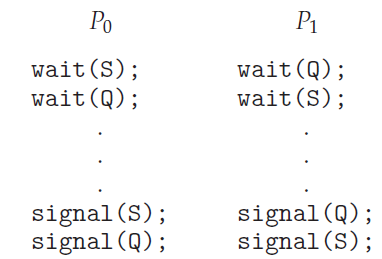
\includegraphics[scale=0.5]{os1.png}
    \caption{Deadlock illustration}
    \label{fig:my_label_1}
\end{figure}

\begin{itemize}
    \item Suppose that $P_0$ executes \texttt{wait(S)} and then $P_1$ executes \texttt{wait(Q)}.When $P_0$ executes \texttt{wait(Q)}, it must wait until $P_1$ executes \texttt{signal(Q)}. 
    
    \item Similarly, when $P_1$ executes \texttt{wait(S)}, it must wait until $P_0$ executes \texttt{signal(S)}. Since these \texttt{signal()} operations cannot be executed, $P_0$ and $P_1$ are deadlocked.
\end{itemize}

\subsection{Priority Inversion}
\begin{itemize}
    \item The situation of \textbf{priority inversion} arises when a higher priority process' access to shared resources is blocked by a lower priority process that holds a lock on the shared resource.
    
    \item For example, if there are three processes L, M and H with priority order $L<M<H$ and L has a lock on resource R. If H desires the resource R then it must wait for L to release the lock. 
    
    \item If L is preempted by M before it can release its lock on R then H is made to wait even longer. 
    
\end{itemize}

\subsubsection{Priority Inheritance Protocol}
\begin{itemize}
    \item This is one possible solution to the Priority Inversion problem.
    
    \item All processes that access a shared resource needed by a higher priority process inherit this higher priority until they release their lock on this resource.
    
    \item Once the lock is released, the priority returns to its normal (lower value).
    
    \item In the above example, L would inherit the priority of H, hence it would not be preempted by M. Hence, after L releases the lock and returns to its original priority, H is the next process to access the shared resource (not M). 
\end{itemize}


\section{Classic Problems in Synchronization}
\subsection{The Bounded-Buffer Problem}

\begin{itemize}
    \item The producer and consumer processes share the following resources:
\end{itemize}

\begin{figure}[!h]
    \begin{minted}{c}
        int n;
        semaphore mutex = 1;
        semaphore empty = n;
        semaphore full = 0;
    \end{minted}
\end{figure}
\begin{itemize}
    \item It is assumed that the pool consists of $n$ buffers each of size 1. 
    
    \item The semaphore variables \texttt{empty} and \texttt{full} count the number of empty and full buffers respectively. 
    
    \item The code for the producer and consumer is given below
\end{itemize}
\begin{figure}[!ht]
 \begin{minipage}{0.5\textwidth}
  \centering
  \begin{minted}{c}
   do{
        next_produced = produce_item();
        
        wait(empty);
        wait(mutex);
        
        add(next_produced, buffer);
        
        signal(mutex);
        signal(full);
   }while(true);
  \end{minted}
  \title{Code for producer process}
 \end{minipage}
 \begin{minipage}{0.5\textwidth}
  \centering
  \begin{minted}{c}
  do{
        wait(full);
        wait(mutex);
        
        next_consumed = remove_item(buffer);
        
        signal(mutex);
        signal(empty);
        
        /* Consume item in next_consumed */
   }while(true);
  \end{minted}
  \title{Code for consumer process}
 \end{minipage}
\end{figure}

\subsection{The Readers-Writers Problem}
\begin{itemize}
    \item Processes are divided into 2 categories: those that only read from a shared memory (readers), and those that only write to the shared memory (writers).
    
    \item The problems arise when readers and writers concurrently try to operate on the same memory, which can lead to the writer overwriting the data which was needed by the writer, or the reader reading an out-of-date value from the memory. 
    
    \item The readers-writers problem has many variations, in particular the \textit{first} and \textit{second} readers-writers problems, which deal with priority order between readers and writers.
    
    \item In the \textbf{first} readers-writers problem, no reader must be kept waiting unless a writer has already obtained permission to access the shared memory.
    
    \item This implies that no reader should wait for other readers to finish simply because a writer is waiting
    
    \item In the \textbf{second} readers-writers problem, once a writer is ready, it should perform the write as soon as possible, without any readers interfering in between. 
    
    \item This implies that if a writer is waiting to access the object, no new readers may start reading.
    
    \item While solving the first problem, writers should not starve. While solving the second problem, readers should not starve. 
\end{itemize}

\subsubsection{Solution to First Readers-Writers Problem}
\begin{itemize}
    \item The reader and writer share the common resources:
\end{itemize}
\begin{figure}[!h]
    \begin{minted}{c}
        semaphore rw_mutex = 1;
        semaphore mutex = 1;
        int read_count = 0;
    \end{minted}
\end{figure}

\begin{itemize}
    \item The \texttt{mutex} semaphore is used to ensure mutual exclusion when the
variable \texttt{read\_count} is updated. 

    \item The \texttt{read\_count} variable keeps track of how many processes are currently reading the object. 
    
    \item The semaphore \texttt{rw\_mutex} functions as a mutual exclusion semaphore for the writers. It is also used by the first or last reader that enters or exits the critical section. It is not used by readers who enter or exit while other readers are in their critical sections.
\end{itemize}

\begin{figure}[!ht]
 \begin{minipage}{0.5\textwidth}
  \centering
  \begin{minted}{c}
   do{
        wait(mutex);
        read_count++;
        if(read_count==1)
            wait(rw_mutex);
        signal(mutex);
        
        /*Perform read operation*/
        
        wait(mutex);
        read_count--;
        if(read_count==0)
            signal(rw_mutex);
        signal(mutex);
   }while(true);
  \end{minted}
  \title{Code for reader process}
 \end{minipage}
 \begin{minipage}{0.5\textwidth}
  \centering
  \begin{minted}{c}
  do{
        wait(rw_mutex);
        
        /* Perform write operation */
        
        signal(rw_mutex);
   }while(true);
  \end{minted}
  \title{Code for writer process}
 \end{minipage}
\end{figure}
\begin{itemize}
    \item If a writer is in its critical section and $n$ readers are queued, then one reader is queued on \texttt{rw\_mutex} while $n-1$ readers are queued on the \texttt{mutex} semaphore. 
    
    \item When a writer executes the \texttt{signal(rw\_mutex)} call, the next executed process may be a single waiting writer or any one of the $n$ waiting readers. This decision is made by the scheduler. 
    
    \item A more general solution of the readers-writers problem involves the use of special \textit{reader-writer} locks in place of mutex/semaphore locks as above. 
    
    \item Readers acquire such a lock in \textit{read} mode, while writers acquire it in \textit{write} mode. 
    
    \item Multiple readers can acquire a lock in read mode, but only one writer can acquire a lock in write mode as writing needs mutual exclusion. 
\end{itemize}

\subsection{The Dining Philosopher's Problem}
\begin{itemize}
    \item There are $n$ philosophers sitting around a table, who spend their entire lives eating or thinking. There are $n$ chopsticks on the table, one between every two philosophers. There is one single bowl of food at the center of the table to be shared by all the $n$ philosophers.
    
    \item A philosopher may pick up only one chopstick at a time. When a hungry philosopher has both chopsticks in hand, they start eating until they are full, without releasing the chopsticks. Once the philosopher is finished eating, they release both chopsticks and resume thinking.
    
    \item The problem statement is to devise a deadlock and starvation free manner in which the philosophers (labelled $1..n$) can pick up the chopsticks and eat. 
\end{itemize}

\subsubsection{Solution to Dining Philosopher's Problem}
\begin{itemize}
    \item The simplest solution is to represent the $n$ chopsticks as an array of semaphores. The act of picking up a chopstick is represented as a \texttt{wait()} and the act of putting it down is represented as \texttt{signal()}.
    
    \item The structure of the ith philosopher is described below:
\end{itemize}

\begin{listing}[!h]
    \begin{minted}{c}
        do{
            wait(chopstick[i]);
            wait(chopstick[(i+1)%n];
            
            /* Eating */
            
            signal(chopstick[i]);
            signal(chopstick[(i+1)%n];
            
            /* Thinking */
            
        }while(true);
    \end{minted}
    \title{Process structure for Dining Philosopher's Problem}
\end{listing}

\begin{itemize}
    \item This solution ensures that no 2 neighbours are eating at once, but if all $n$ philosophers are hungry at once and all pick up the chopstick to their left then they will be stuck in a \textbf{deadlock} waiting for the neighbour to release their chopstick.
    
    \item Some possible remedies to the deadlock problem are:
    \begin{itemize}
        \item Allow a philosopher to eat only if both chopsticks are avaiable. This turns the eating into a critical section.
        
        \item Using an asymmetric solution where an odd-numbered philosopher first picks up the left then the right chopstick, but the even-numbered philosopher first picks up the right then the left chopstick. 
    \end{itemize}
\end{itemize}

\section{Examples of Process Synchronization}
\subsection{Windows Synchronization}
\begin{itemize}
    \item On a single processor system, the Windows kernel temporarily masks all interrupts that can access shared resources. 
    
    \item On multiprocessor systems, shared resources are protected by the kernel using spinlocks (only for short code segments). The kernel ensures that threads will never be preempted while they hold a spinlock.
    
    \item Outside of the kernel, Windows uses \textbf{dispatcher objects} for synchronization. 
    
    \item Dispatcher objects provide many different methods for synchronization such as mutexes, semaphores, events (condition variables) and timers (used to notify one or more threads that a certain time has elapsed).
    
    \item Dispatcher objects may be in \textbf{signaled} state or \textbf{nonsignaled} state. In signaled state, a thread will not block while taking control of the object, while in nonsignaled state, threads will block while attempting to take control of the dispatcher object. 
    
    \item When a thread blocks on a nonsignaled dispatcher object, it is placed into the waiting queue from the ready queue. 
    
    \item When the dispatcher object moves to signaled state, the kernel checks if any threads are waiting for it. If there are such threads, they are moved from the waiting to the ready queue
    
    \item Windows also provides \textbf{critical-section objects} which are user-mode mutexes.
    
    \item On a multiprocessor system, a critical-section object first uses a spinlock while waiting for the other thread to release the object. If it spins too long, the acquiring thread will then allocate a kernel mutex and yield its CPU.
    
    \item Critical-section objects are particularly efficient because the kernel mutex is allocated only when there is contention for the object. In practice, there is very little contention, so the savings are significant.
\end{itemize}

\subsection{Linux Synchronization}
\begin{itemize}
    \item The simplest synchronization technique in Linux is the use of atomic data types that allow operations (for example math operations on integers) to be done entirely atomically. 
    
    \item Linux also provides spinlocks, mutex locks and semaphores as mechanisms on multi-processor systems
    
    \item On single processor machines (eg: embedded systems), Linux allows disabling and enabling kernel preemption in place of acquiring and releasing a lock. This is done using two system calls \texttt{preempt\_disable()} and \texttt{preempt\_enable()}
    
    \item Every process contains a \texttt{thread\_info} structure which contains one counter (called \texttt{preempt\_count}) for the number of locks being held by the task, which is incremented or decremented as a lock is acquired or released respectively. 
    
    \item If \texttt{preempt\_count} is greater than 0, then it is not safe for the task running to be preempted, but if it is 0 then the task can be safely preempted. 
\end{itemize}

\subsection{pthread Synchronization}
\begin{itemize}
    \item The \texttt{pthread} API provides a user-accessible implementation of synchronization structures independent of the kernel for POSIX-compliant systems.
    
    \item Mutex locks are provided using the \texttt{pthread\_mutex\_t} data structure and initialized using the \texttt{pthread\_mutex\_init()} function. 
    
    
    \item They can be acquired and released using the \texttt{pthread\_mutex\_lock()} and \texttt{pthread\_mutex\_unlock()} functions respectively. 
    
    \item Semaphores (part of a separate semaphore API) are declared using the \texttt{sem\_t} data structure, and initialized using the \texttt{sem\_init()} function. 
    
    \item The wait and signal operations of semaphore are implemented as the \texttt{sem\_wait()} and \texttt{sem\_post()} functions respectively. 
    
    \item The semaphore API provides \textbf{named} and \textbf{unnamed} semaphores. The difference is that named semaphores have file system names and can be accessed across multiple unrelated processes. Unnamed semaphores can only be accessed by threads belonging to one single process. 
\end{itemize}

\section{Deadlocks}
\subsection{System Model}
\begin{itemize}
    \item The set of available resources in the system is modelled as belonging to different classes. 
    
    \item In each class of resources $R_i, i \in \{1, 2, ..., n\}$, there are $W_i$ instances, all of which are \textbf{entirely identical}. 
    
    \item A process undertakes resource utilization in the following order
    \begin{enumerate}
        \item \textbf{Request} for access. If not immediately available then wait
        
        \item \textbf{Use} the resource
        
        \item \textbf{Release} the resource for use by others
    \end{enumerate}
\end{itemize}
\subsection{Necessary Conditions}
The follwing conditions must simultaneously hold for a situation to be characterized as a deadlock. 
\begin{itemize}
    \item \textbf{Mutual Exclusion}: At least one resource is held by a process and cannot be shared with other processes (other processes have to wait for it to be released)
    
    \item \textbf{Hold and Wait}: A process that currently holds resource $R_1$ is waiting for another resource $R_2$ that is being currently held by some other process.
    
    \item \textbf{No Preemption}: Resources can only be released if the process voluntarily releases them itself. No external process (not even the kernel) can preempt the process and force it to give up the lock on the currently held resource.
    
    \item \textbf{Circular Waiting}: There exists a set of process $P_1, P_2, ..., P_n$ such that $P_1$ is waiting for a resource held by $P_2$, $P_2$ is waiting for a resource held by $P_3$, $P_3$ is waiting for a resource held by $P_4$, and so on, and $P_n$ is waiting for a resource held by $P_1$. 
\end{itemize}

\subsection{Resource Allocation Graph}
\begin{itemize}
    \item The allocation of resources to processes is visualized by a graph.
    
    \item The vertices are of two types, the active processes (circles) and the resource classes in the system (rectangles). Instances of the same resource class are denoted as dots within the rectangle of that resource class. 
    
    \item There are two types of edges, the request edge (directed from process $P_i$ to resource class $R_j$) and the assignment edge (directed from resource class $R_j$ to process $P_i$).
\end{itemize}
\begin{figure}[h]
    \centering
    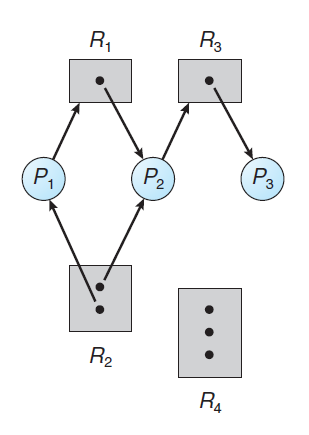
\includegraphics[scale = 0.7]{os2.png}
    \caption{Resource Allocation Graph}
    \label{fig:my_label_yy}
\end{figure}

\begin{itemize}
    \item If the graph contains no cycles, then there are no deadlocks in the system.
    
    \item If the graph contains a cycle, there \textit{may be} a deadlock.
    
    \item If all resource types have only one instance, then a cycle implies a deadlock has occurred. In this case, the existence of a cycle is necessary and sufficient condition for deadlock to exist.
    
    \item But if resource types in the cycle have multiple instances, then cycle does not necessarily imply a deadlock. 
\end{itemize}

\subsection{Methods for Handling Deadlocks}
\begin{itemize}
    \item The following methods may be used to avoid deadlocks:
    \begin{itemize}
        \item Deadlock prevention (preventing the system from entering a deadlocked state under any circumstance)
        
        \item Allow the system to enter a deadlock state, detect it and then recover from it.
        
        \item Ignore the existence of deadlocks and continue normal operation (used in Windows and Linux). This places the responsibility of deadlock avoidance on the application programmer. 
    \end{itemize}
\end{itemize}

\section{Deadlock Detection}
\begin{itemize}
    \item In a system where each resource class has only one instance, deadlocks are detected from the \textbf{wait graph}.
    
    \item The wait graph is constructed from the resource allocation graph, where each vertex denotes a process and an edge from $P_i$ to $P_j$ denotes that $P_i$ is waiting for $P_j$.
    
    \item A cycle in the wait graph denotes the existence of a deadlock, and detecting a cycle in the graph is an $O(n^2)$ process where $n$ is the number of processes (ie. vertices) in the graph. 
    
\end{itemize}
\begin{figure}[h]
    \centering
    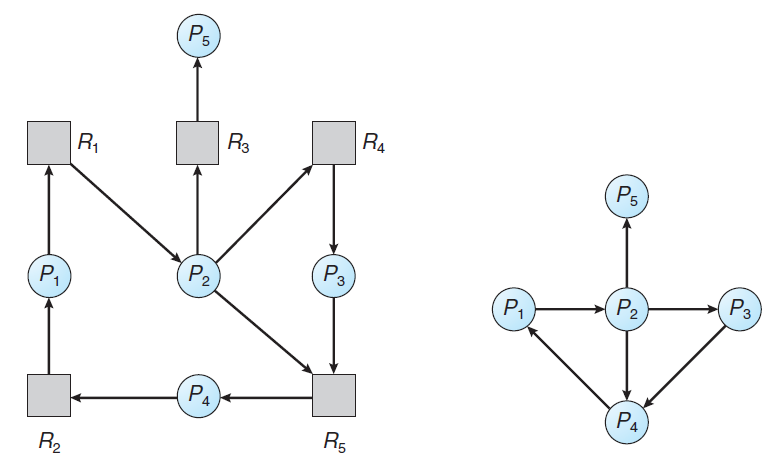
\includegraphics[scale = 0.5]{os3.png}
    \caption{Resource Allocation Graph and the corresponding Wait Graph}
    \label{fig:my_label_xxx}
\end{figure}
\subsection{Multiple Instance per Resource Class}
\begin{itemize}
    \item Let there be $m$ resource classes and $n$ active processes in the system. 
    
    \item The algorithm used to detect a deadlock in such a situation makes use of the following data structures:
    \begin{itemize}
        \item \textbf{Available}: A vector of length $m$ indicating the number of resources available per resource class.
        
        \item \textbf{Allocation}: An $n \times m$ matrix which denotes the number of instances of each resource class allocated to each process. 
        
        \item \textbf{Request}: An $n \times m$ matrix which denotes a request made by a process for a resource instance. If $R[i][j] == k$ then process $R_i$ is requesting $k$ instances of resource class $R_j$. 
    \end{itemize}
\end{itemize}

\subsubsection{Algorithm for Deadlock Detection}
\begin{enumerate}
    \item Let \texttt{work} and \texttt{finish} be vectors of length $m$ and $n$ respectively. Initialize \texttt{work = available}. For $i \in \left[0, n-1\right]$ if \texttt{allocation[i] $\ne 0$,} \texttt{finsh[i]=false} else \texttt{true}.
    
    \item Find an index \texttt{i} such that \texttt{finish[i] == false} and \texttt{request[i] $\le$ work}. If no such \texttt{i} exists, go to step 4
    
    \item Set \texttt{work = work + allocation} and \texttt{finish[i] = true}. Go to step 2
    
    \item If \texttt{finish[i] == false} for some $i \in \left[0, n-1 \right]$, then system is in a deadlocked state. Process $P_i$ is in a deadlock. 
\end{enumerate}

\section{Deadlock Prevention}
\subsection{Mutual Exclusion}
\begin{itemize}
    \item Some files (such as read-only files) do not require any mutual exclusion privileges
    
    \item But other resources may require control to ensure no race conditions, 
\end{itemize}

\subsection{Hold-and-Wait}
\begin{itemize}
    \item To ensure that hold and wait does not occur in the system, the OS must make sure that when a process requests for a resource, it is not holding any other resources. 
    
    \item One such protocol to implement this is the process requesting for all of its resources at the very beginning and getting all of them at that time. 
    
    \item This is done by forcing all system calls for resource allocation to come before any other system calls.
    
    \item Another protocol is to allocate resources to a process only if that process is not holding any other resources. If it is holding any other resources it must release them before asking for more resources.
    
    \item Both protocols here suffer from the problem of starvation (processes asking for popular resources may have to wait infinitely) and low resource utilization (due to resources being allocated and not used by processes)
\end{itemize}

\subsection{No Preemption}
\begin{itemize}
    \item If a process holding some resources asks for another resource which is currently not available, then all the currently held resources may be released and added to the list of resources requested by that process
    
    \item Then the process must wait until both old and new resources are available for the process to acquire. 
    
    \item An alternate approach is to allocate resources to a process $P_1$ that asks for them if they are available.
    
    \item If the resources are being held by another process $P_2$ that is, in turn, requesting for another resource, then we preempt the desired resources from the waiting process $P_2$ and allocate them to the requesting process $P_1$. 
    
    \item If the resources are neither available nor held by $P_1$, the requesting process must wait. While it is waiting, some of its resources may be preempted, but only if another process requests them
    
    \item The second protocol is applied to resources that can be saved and restored later (like CPU registers and memory), but not to resources like mutex locks/semaphores.
\end{itemize}

\subsection{Circular Waiting}
\begin{itemize}
    \item Let there be the resource classes $\{ R_1, R_2, ..., R_m\}$ each with its own unique integer value, given by the function $f(R_i)$. 
    
    \item A process can only request the resources if the requests are made in an increasing order of this function $f$. For example, a request for resource class $R_j$ can be made after a request for class $R_i$ only if $f(R_i) < f(R_j)$
    
    \item Alternatively, a process that requests a resource class $R_j$ must free all instances of resource class $R_i$ such that $f(R_j) \ge f(R_i)$
    
    \item All the applications written by third party programmers must also conform to this ordering to avoid deadlocks.
    
    \item The function $f$ must be chosen in such a way that it follows the real-world usage order of system resources. 
    
    \item Deadlocks can be prevented by using system utilities like \textbf{witness} (on BSD UNIX systems) that determines the order of locks taken in the system and checks for a deadlock possibility if locks are held out of order. 
\end{itemize}
\end{document}